\documentclass{homework}

\title{Homework 11}
\author{Kevin Evans}
\studentid{11571810}
\date{April 19, 2020}
\setclass{Physics}{304}
\usepackage{amssymb}
\usepackage{mathtools}

\usepackage{amsthm}
\usepackage{amsmath}
\usepackage{slashed}
\usepackage{relsize}
\usepackage{threeparttable}
\usepackage{float}
\usepackage{booktabs}
\usepackage{boldline}
\usepackage{changepage}
\usepackage{physics}
\usepackage[inter-unit-product =\cdot]{siunitx}
\usepackage{setspace}

\usepackage[makeroom]{cancel}
\usepackage{pgfplots}

\usepackage{multicol}
\usepackage{tcolorbox}
\usepackage{enumitem}
\usepackage{times}
\usepackage{mhchem}
\usepackage{graphicx} 
\DeclareSIUnit{\year}{yr}
\usepackage[export]{adjustbox}

\usepackage{dsfont}
\newcommand{\1}{\mathds{1}}

\begin{document}
	\maketitle
	\subsubsection*{State vectors and Dirac brackets}
	\begin{enumerate}[label={\arabic*.}]
		\item Because $\braket{e_n}{e_m} = \delta_{nm}$, when you take $\braket{e_n}{V}$, it takes the coefficient of only the $\ket{e_n}$ component of $V$, as $\delta_{nm} = 1$ for $n=m$. The other components are zeroed out.
		
		\item Starting from ($6$), \begin{align*}
			\1\ket{V} & = \sum_n \ket{e_n} \braket{e_n}{V} \\
				& = \sum_n a_n \ket{e_n} \\
				& = \ket{V} \qed
		\end{align*}
	
		\item For an infinite square well of length $L$, the normalized wavefunction is given as \begin{align*}
			\ket{\Psi_n} & = \sqrt{ \frac{2}{L} } \sin(\frac{ n \pi x}{L}) \qquad n \in \mathbb{Z}
			\intertext{If we take the inner product of two states, then}
			\braket{\Psi_n}{\Psi_m} & = \int_\mathbb{R} \Psi_n^*(x) \Psi_m(x) \dd{x}
			\intertext{Recognizing that $\Psi(x) \in \mathbb{R} \; \forall \; n, m \in \mathbb{Z}$ and the wavefunctions must be zero outside the interval $[0, L]$, we can limit the integral bounds and remove the conjurgation,}
			\braket{\Psi_n}{\Psi_m} & = \int_{0}^{L} \Psi_n(x) \Psi_m(x) \dd{x} \\
				& = \frac{2}{L} \int_{0}^{L} \sin(\frac{n \pi x}{L}) \sin(\frac{m \pi x}{L}) \dd{x} \\
				& = \frac{1}{L} \int_{0}^{L}
					\left[
						\cos( \frac{(n-m) \pi x}{L}  )
						- \cos( \frac{(n + m) \pi x}{L} )
					\right] \dd{x}
			\intertext{As $(n \pm m) \in \mathbb{Z}$ (closure under addition), then the integral must be zero for $m \ne n$ as we are integrating over equal parts. For $n=m$, the first cosine evaluates to $L$ and the second evaluates to zero. Then, }
			\braket{\Psi_n}{\Psi_m} & = \begin{cases*}
				0 & $m \ne n$ \\
				1 & $m = n$
			\end{cases*} \\
			& = \delta_{mn} \text{, these states form an orthonormal basis.} \qed
		\end{align*}
	
		\pagebreak
		\item From ($8$), \begin{align*}
			\braket{\phi}{\Psi} & = \int_\mathbb{R} \overline{\phi(x)} \Psi(x) \dd{x}
			\intertext{If we take the conjurgation of the RHS, it can be shown}
			\overline{\int_\mathbb{R} \overline{\phi(x)} \Psi(x) \dd{x}} & = \int_\mathbb{R} \phi(x) \overline{\Psi(x)} \; \overline{\dd{x}} \\
				& = \int_\mathbb{R} \overline{\Psi(x)} \phi(x) \dd{x} && \text{As $\overline{\dd{x}} = \dd{x}$ since $x \in \mathbb{R}$} \\
				& = \braket{\Psi}{\phi} \qed
		\end{align*}
	
		\item If we let $\alpha = 2\pi / L$, then \begin{align*}
			\braket{\phi_n}{\phi_m} & = \frac{1}{L} \int_\mathbb{R} e^{-i \alpha n x} e^{i\alpha m x} \dd{x} \\
				& = \frac{1}{L} \int_0^L e^{i \alpha x (m-n)} \dd{x}
			\intertext{For $m = n$,}
				\braket{\phi_n}{\phi_m} & = \frac{1}{L} \eval{x}_{0}^L = 1
			\intertext{For $m \ne n$, if we expand the exponential using Euler's formula, the integrals must evaluate to zero, since the evaluation subtracts integral multiples of an entire sinusodial cycle, i.e. it's zero since}
				\cos(2\pi k) & = 1, \\
				\sin(2\pi k) & = 0 \qquad  \forall \;k \in \mathbb{Z} \\
			\braket{\phi_n}{\phi_m} & = \delta_{mn} \qed	
		\end{align*}
		\pagebreak
		\item \begin{enumerate}
			\item It's normalized as the probability for $0 < x < L/2$ is given as \begin{align*}
				P(x) & = \Psi(x) * \Psi(x) = 2/L \\
				1 & = \eval{\frac{2}{L} x}_{0}^{L/2} \text{ is true}
			\end{align*}
		
			\item By definition, \begin{align*}
				\ket{\Psi(x)} & = \sum_n a_n \ket{\phi_n} \\
				%\ket{\Psi(x)} & = \frac{1}{L} \sum_n a_n e^{2 \pi i n x / L}
				\intertext{If we take $\braket{\phi_m}{\cdot}$ on both sides, where $\ket{\phi_m}$ is an arbitrary element of the basis, then the RHS will reduce to a single element in the summation (as shown in Problem 5),}
				\braket{\phi_m}{\Psi} & = \sum_n a_n \braket{\phi_m}{\phi_n} \\
				\int_{\mathbb{R}} \phi_m^*(x) \Psi(x) \dd{x} & = \sum_n a_n \delta_{mn} = a_m \\
				\intertext{Reducing the bounds from $\mathbb{R} \to [0, L/2]$ and renaming $m\to n$,}
				a_n & = \int_0^{L/2} \frac{1}{\sqrt{L}} e^{-2\pi i n x / L} \sqrt{\frac{2}{L}} \dd{x} \\
				& = -\frac{i\left(1 - e^{-in\pi}\right)}{\sqrt{2}n\pi} && \text{Evaluated using WolframAlpha}
				\intertext{Since $1-e^{-in\pi} = 0$ for $n = \text{even integers}$, the summation becomes}
				\ket{\Psi(x)} & = \sum_{n = \mathrm{odd}} -\frac{i\left(1 - e^{-in\pi}\right)}{\sqrt{2}n\pi} \ket{\phi_n}
			\end{align*}
		\end{enumerate}
	
		\item From the completeness, \begin{align*}
			\braket{\Psi}{\Psi} = \bra{\Psi} \1 \ket{\Psi} & = \bra{\Psi} \sum_n a_n \ket{\phi_n} \\
				& = \sum_n a_n \braket{\Psi}{\phi_n} \\
				& = \sum_n \left(a_n\right)^2 \qed
		\end{align*}
	
		\item I think I must've messed up in Problem 6, so I'm going to just omit the exponential term and use \begin{align*}
			a_n & = -\frac{i}{\sqrt{2} n \pi} \\
			\hat{P}\ket{\phi_n} & = \sum_n \abs{a_n}^2 = \sum_n \frac{1}{2 \pi^2 n^2} \\
				& = \frac{1}{2 \pi^2} \times \frac{ \pi^2 }{4} \\
				& = \frac{1}{8} \leftarrow \text{Definitely not right...}
		\end{align*}
	
		\item Assuming $a$ and $b$ are matrices as well, it iterates over the rows in $a$, takes the product of $M_{nm}$ and $a_m$ for every element in $a$. Then that row is summed and stored in $b_n$. Maybe?
		
		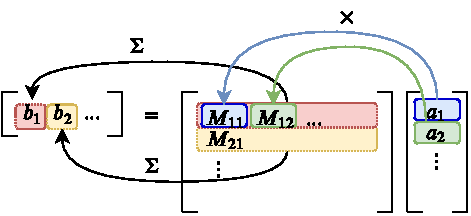
\includegraphics{hw11mtx}
		
		\item From applying the completeness twice, \begin{align*}
			\ket{\Phi} & = \hat{A} \ket{\Psi} \\
			 & = \hat{A} \left[\1 \ket{\Psi} \right] \\
			 & = \1 \left[ \hat{A} \sum_m a_m \ket{\phi_m} \right] \\
			 & = \sum_{n} \sum_m a_m \ket{\phi_n} \underbrace{\bra{\phi_n} \hat{A} \ket{\phi_m}}_{A_{nm}} \\
	 \sum_n b_n \ket{\phi_n} & = \sum_{n} \sum_m a_m \ket{\phi_n} A_{nm} && \text{Equating the inner parts} \\
	 	b_n & = \sum_m A_{nm} a_m
		\end{align*}
	\end{enumerate}
\end{document}